\documentclass[linenumbers,twocolumn]{aastex631}
% \documentclass[linenumbers]{aastex631}

% Packages
\usepackage[utf8]{inputenc}
\usepackage{graphicx}
\usepackage{amsmath}
\usepackage{amssymb}
\usepackage{enumitem}
\usepackage{ulem}
\usepackage{hyperref}

% Editing commands
\newcommand{\mm}[1]{{\textcolor{purple}{\bf #1}}}

% Make upright subscripts and superscripts in Mathmode.
\def\subinrm#1{\sb{\mathrm{#1}}}
{\catcode`\_=13 \global\let_=\subinrm}
\mathcode`_="8000
\def\supinrm#1{\sp{\mathrm{#1}}}
{\catcode`\^=13 \global\let^=\supinrm}
\mathcode`^="8000
\def\upsubscripts{\catcode`\_=12 } \def\normalsubscripts{\catcode`\_=8 }
\def\upsupscripts{\catcode`\^=12 } \def\normalsupscripts{\catcode`\^=7 }

\newcommand{\vdag}{(v)^\dagger}
\newcommand\aastex{AAS\TeX}
\newcommand\latex{La\TeX}

% Title
\shorttitle{Deriving the Shock Crossing Time}
\shortauthors{Moss M.} 

\begin{document}

\upsubscripts
\upsupscripts

\title{Deriving the Shell Crossing Time as a Function of the Density}

\correspondingauthor{Michael Moss}
\email{mikejmoss3@gmail.com}

\begin{abstract}
The goal of this derivation to estimate the time it will take a reverse shock to cross incoming ejecta material.

\end{abstract}

\section{Introduction}
{
    In the refreshed shock model, the wind of a GRB can be separated into two regions, (i) early outflow launched with $\bar{\Gamma}\sim100$ and (ii) later ejecta launched launched with $\bar{\Gamma}\sim10$. The early material is responsible for producing the prompt emission and the afterglow continuum emission. The later ejecta will eventually catch up to the early ejecta as it sweeps up circumburst medium and decelerates. When the later ejecta catches up and collides with the early material, a ``refreshed'' shock occurs, injecting energy into the front of the outflow and may be witnessed as bumps in the afterglow light curves (potentially in the optical regime). In this work, we would like to estimate the time it takes the incoming energy injected from the later ejecta to be distributed across the newly shocked material. This timescale should be dominated by the shell crossing time $\Delta t_{shell}$, where we model the incoming late ejecta as a shell with mass $M_{r}$ and Lorentz factor $\Gamma_{r}$ (see Figure \ref{fig: schematic}).

    \begin{figure*}[t!]
        \centering
        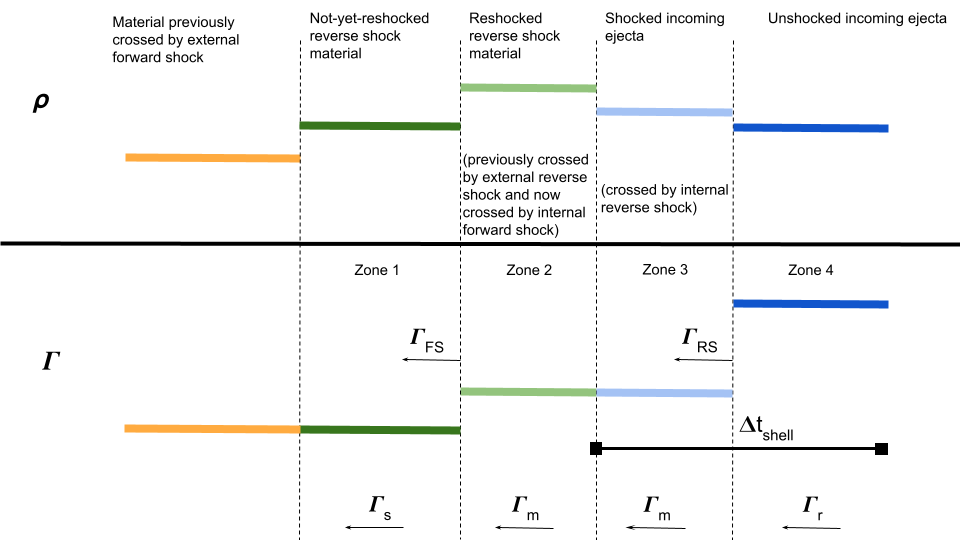
\includegraphics[width=0.8\textwidth]{schematic.png}
        \caption{Schematic of the scenario (in the central engine frame). There are two ``reverse shocks'' in question. The reverse shock arising from the bulk of the jet decelerating as it sweeps up circumburst medium, which will be referred to as the external reverse shock. And an internal revers shock arising from the deceleration of the incoming later ejecta decelerating as it rams the material in front of it (which happens to be the material previously crossed by the external reverse shock).}
        \label{fig: schematic}
    \end{figure*}

    To estimate the time it will take for an internal reverse shock to cross incoming material, we must estimate the density in the slow material (zone 1 material) and the rapid material (zone 4 material). 
}

% \section{Estimating Density of the Outflow Material}
% {
%     The average mass density of the material, $\rho$, in the bulk GRB outflow (in the central engine frame) can be found using the isotropic equivalent energy injection rate, $\dot{E}_{iso}$, 

%     \begin{align}
%     \dot{E}_{iso} &= \dot{M}_{iso} \Gamma_{s,0} c^2\\
%     &\text{where } \dot{M}_{iso} = 4 \pi c R^2 \rho\\
%     \Rightarrow \rho &= \frac{\dot{E}_{iso}}{4\pi \Gamma_{s,0} c^3 R^2}
%     \end{align}

%     where $R$ is the radius out to the point of collision, $M_{iso}$ is the isotropic equivalent mass injection jet, and $\Gamma_{s,0}$ is the average bulk Lorentz factor of the early ejecta before deceleration. 

%     We can estimate the density using the fiducial values $\dot{E}_{iso} = 10^{53}$ erg/s, $R=10^{17}$ cm, and $\Gamma_{s,0} = 100$, which results in a density of $\bar{\rho}_{jet}\approx 3\times10^{-16}$ g cm$^{-3}$ ($n \approx 2\times 10^{8}$ cm$^{-3}$; central engine frame). This is very uncertain and most likely a large underestimation of the true density in the merging material.
% }


\section{The Width of the Incoming Ejecta}
{
    The width of the late ejecta at the location of the refreshed shock, i.e., $R = R_{coll} \approx 10^{17}$ cm, can be approximated using the isotropic equivalent energy of the late material in zone 4 $E_{iso,4}$  and assuming some density of the material,

    \begin{align}
        M_{iso,4} &= 4 \pi R^2 \rho_{4} \ell\\
        % \frac{E_{iso,4}}{\Gamma_r c^2} &= 4\pi R^2 \rho_{4} \ell\\
        \Rightarrow \ell &= \frac{E_{iso,4}}{4\pi\Gamma_r R^2 c^2 \rho_{4}}
    \end{align}

    where $\rho_{4}$ and $\Gamma_r$ are the mass density at radius R and Lorentz factor of the late material in zone 4, respectively. In our model, we keep the isotropic equivalent energy injection rate constant, so $E_{iso,4}$ can be approximated as $E_{iso,4} = \dot{E}_{iso} * \Delta t_{late}$ erg, where $\Delta t_{late}$ is the duration of the late material responsible for the refreshed shock, which, in this example, is close to half the total duration of the wind (e.g., $\sim$ 15 seconds).
}

\section{Shell Crossing Time}  
{
    In the central engine frame, the shell crossing time can be defined as

    \begin{align}
        \Delta t_{shell} = \ell \frac{2\Gamma_{RS}^2\Gamma_{r}^2}{c(\Gamma_{r}^2 - \Gamma_{RS}^2)}
    \end{align}

    where $\ell$ and $\Gamma_{r}$ are the width and bulk Lorentz factor of the late ejecta material, $\Gamma_{RS}$ is the Lorentz factor of the reverse shock, where $\Gamma_r > \Gamma_{RS}$ (see Figure \ref{fig: schematic}; Kobayashi et al 1997). In the observer frame this duration is reduced by a factor of $1/2\Gamma_m^2$, where $\Gamma_m$ is the resulting bulk Lorentz factor of the merged material and can be approximated as 

    \begin{align}
        \Gamma_m \approx \sqrt{\Gamma_{r}\Gamma_{s}}\sqrt{\frac{m_{r}\Gamma_{r} + m_{s}\Gamma_{s}}{m_{r}\Gamma_{s} + m_{s}\Gamma_{r}}}
    \end{align}

    where $m_{r} = E_{iso,4}/c^2\Gamma_r$ and $m_{s} = E_{iso,1}/c^2\Gamma_s$ are the masses of the ejecta (zone 4) and reverse shock materials (zone 1), respectively, such that,

    \begin{align}
        \Gamma_m \approx \sqrt{\Gamma_{r}\Gamma_{s}}\sqrt{\frac{E_{iso,4} + E_{iso,1}}{E_{iso,4} \Gamma_{s}/\Gamma_{r} + E_{iso,1} \Gamma_{r}/\Gamma_{s}}}
    \end{align}

    Again, in this approximation, we keep the energy injection rate constant and separate the duration of the wind evenly between the early and late ejecta. This means that $E_{iso,1}\approx E_{iso,4}$ and the above expression can be simplified to be 

    \begin{align}
        \Gamma_m &\approx \sqrt{\Gamma_{r}\Gamma_{s}}\sqrt{\frac{2}{\Gamma_{s}/\Gamma_{r} + \Gamma_{r}/\Gamma_{s}}} \\
        & \approx \Gamma_r\Gamma_s \sqrt{\frac{2}{(\Gamma_r^2 + \Gamma_s^2)}}
    \end{align}    

    The Lorentz factor of the reverse shock traveling through zone 4, $\Gamma_{RS}$, can be approximated as 

    \begin{align}
        \Gamma_{RS} \approx \Gamma_m \sqrt{\left(1 + \frac{2\Gamma_m}{\Gamma_r}\right)/\left(2+\frac{\Gamma_m}{\Gamma_r}\right)}
    \end{align}

    See Figure \ref{fig: plot} for a plot of the ejecta shell width and shock crossing times (observer frame) as a function of the material density (assuming values of $\Gamma_{r}=15$, $m_{r}=10^{31}$ g, $\Gamma_{RS}=5$, and $m_{RS}=10^{30}$ g) . 

    We know the estimated density is an underestimation, so the true density will most likely be above the estimate value found above (i.e., above the orange, dotted line in Figure \ref{fig: plot}), which means that the width of the shell is most likely $l_{ej}\lesssim 7\times 10^{12}$ cm and the shock crossing time $\Delta t_{shock} \lesssim 50$ seconds.

    \begin{figure}[t!]
        \centering
        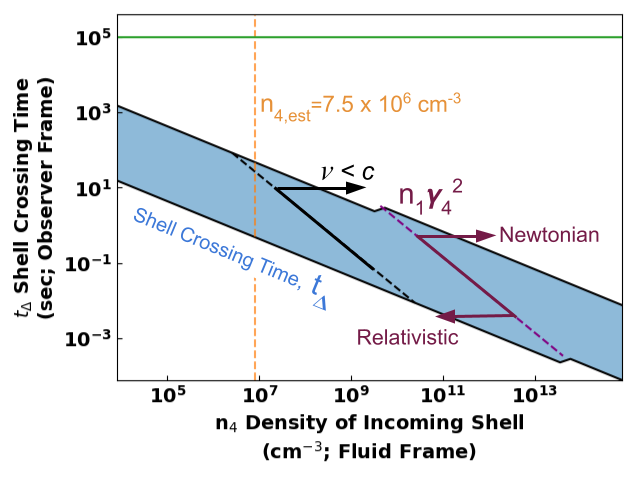
\includegraphics[width=0.45\textwidth]{shell-cross-time.png}
        \caption{Displayed is the ejecta shell width $\ell$ (central engine frame) and shell crossing times $\Delta t_{shell}$ (observer frame) as a function of the mass density of the late ejecta, $n_{late}$. The blue dashed line indicates $t=10^5$ seconds. The orange dotted line is the estimated particle density calculated above. The green, dashed-dotted line indicates if the collision occurs in an ultrarelativistic regime (below) or a Newtonian regime (above).}
        \label{fig: plot}
    \end{figure}
}



\end{document}
